\documentclass[onecolumn]{aastex63}
\usepackage{natbib}
%\definecolor{orcidlogocol}{HTML}{A6CE39}
\bibliographystyle{aasjournal}

\begin{document}

\title{COLLISION RATES OF PLANETESIMALS NEAR MEAN-MOTION RESONANCES}

\author{Spencer C. Wallace}
\affiliation{Astronomy Department, University of Washington, Seattle, WA 98195}

\author{Aaron C. Boley}
\affiliation{Department of Physics and Astronomy, University of British Columbia, Vancouver BC, Canada}

\author{Thomas R. Quinn}
\affiliation{Astronomy Department, University of Washington, Seattle, WA 98195}

\begin{abstract}
In circumstellar disks, collisional grinding of planetesimals produces second-generation dust, which can be observed through thermal 
emission. While it remains unclear when second-generation dust first becomes a major component of the total dust content, the presence of 
such dust and potentially the substructure within it can be used to explore a disk's physical conditions. A perturbing planet has been shown to 
produce nonaxisymmetric structures, as well as gaps in disks, regardless of the origin of the dust. However, small grains will have very 
different dynamics compared with planetesimals when in the presence of gas, and as such, the collisional evolution of planetesimals could 
create dusty disk structures that would not exist otherwise. In particular, mean motion resonances (MMRs) are extremely nonlinear and could 
drive disk morphologies. We use a direct N-body model to track collision rates in a planetesimal disk under the gravitational influence of an 
external Jupiter-sized planet. We show that a perturbing planet can produce significant variations in the collision rate of planetesimals near the 
MMRs and we explore how the mass and eccentricity of the perturbing planet alters this structure. Finally, we use the CASA image simulator to 
predict what the dust emission sturcture should look like with ALMA and the NG-VLA. Although the dust structure produced by MMRs cannot 
be used to directly measure the properties of the perturbing planet, we show that it can be used to place constraints on its mass and 
eccentricity.
\end{abstract}

\section{Introduction} \label{sec:intro}

Recent observations of circumstellar disks by ALMA have revealed a rich variety of substructure in the millimeter wavelength
contiunuum emission. Features such as gaps and asymmetries 
\citep{2015ApJ...808L...3A, 2016Sci...353.1519P, PhysRevLett.117.251101, 2016ApJ...820L..40A, 2016Natur.535..258C} in the 
emission provide diagnostics for the physical processes that drive the evolution of the disks. At these wavelengths, much of this light 
is produced by second-generation debris generated through collisional grinding of planetesimals
\citep[see][]{2008ARA&A..46..339W}. 

In some cases, these gap features are argued to be an indicator for the presence of a giant planet, either embedded in the disk 
\citep{2015MNRAS.453L..73D} or orbiting externally. An giant perturber can influence the structure of the dust emission in a number 
of ways. A misaligned giant planet can produce nonaxisymmetric features such as warps \citep{2001A&A...370..447A}. Highly 
eccentric perturbers can produce even more complicated structures through secular perturbations \citep{2014MNRAS.443.2541P, 
2015MNRAS.448.3679P}. Mean motion resonances (MMRs) have been shown to open gaps as well
\citep{2015ApJ...798...83N, 2016ApJ...818..159T, 2018ApJ...857....3T}.

The dynamics governing the motion of bodies near MMRs is extremely nonlinear, as is determining what the collision rates between 
planetesimals should look like in these regions. For a collection of bodies massive enough to experience the effects of gravitational 
focusing, a large eccentricity dispersion tends to reduce the probability of collision, while enhancements in surface density tends to 
increase it. Due to conservation of the Jacobi energy, MMRs simultaneously enhance the local eccentricity dispersion and also 
enhance the surface density adjacent to the resonance \citep{2000Icar..143...45R, 2017ApJ...850..103B}.

Because the second generation dust production is driven by the planetesimal collision rate, it is crucial to understand how the 
dynamics that drive collisions works. In particular, it is not obvious how to link the readily observable thermal emission from dust in 
protoplanetary disks to the presence of a perturbing giant planet. Due to its nonlinearity, this problem is best studied with N-body 
simulations. Unfortunately, collision detection in an N-body simulation is extremely computationally expensive. So far, studies of 
planetesimal dynamics near MMRs have involved either collisionless test particles \citep{2017ApJ...850..103B, 2016ApJ...818..159T, 
2018ApJ...857....3T} or severely limited integration times \citep{2000Icar..143...45R}.

To further elucidate this subject, we use the tree based N-body code {\sc ChaNGa}
\citep{2008IEEEpds...ChaNGa, 2015AphCom..2..1} to follow the collisional evolution of a planetesimal disk under the gravitational 
influence of a Jupiter sized body. Because particle positions are sorted into a tree structure, neighbor finding and collision detection 
can be done quickly and efficiently. This considerably relaxes the constraints on resolution and integration time. With this toolset, we 
explore the collision rate structure of the planetesimal disk in the vicinity of mean motion resonances. In particular, we would like to 
determine: 1. whether MMRs leave a detectable signature in the collisionally-generated dust. 2. If these signatures can be used to determine the orbital properties of the perturbing planet.

This work is organized in the following way: In section \ref{sec:dynamics}, we provide an overview of the relevant dynamics that drive 
the evolution of a planetesimal disk under the gravitational influence of an external perturber. We also highlight the shortcomings of secular theory in trying to predict the radial collision rate and motivate the need for N-body simulations with massive, collisional particles. In section \ref{sec:sims} we describe the N-body code that we use and detail the initial conditions that are used for two simulations: one in which the perturber is on a circular orbit and another in which the perturber is given a mildly eccentric orbit. Section \ref{sec:results} presents the results of the two simulations. Next, we generate dust emission maps in section \ref{sec:dust}, under the assumption that collisionally-generated dust will quickly couple with the gas and circularize, and show that radial structure is produced in the vicinity of the MMRs. Using the dust emission maps, section \ref{sec:fitting} explores the feasibility of measuring properties of the perturbing planet from the MMR features in the dust. We then conclude in section \ref{sec:discuss}. 

\section{Overview of Relavant Dynamics} \label{sec:dynamics}

\subsection{Collision Rates of Massive Bodies}

We begin by making the assumption that a typical encounter between planetesimals in a disk is well-described by two-body 
dynamics. So long as the random velocities of planetesimals $v_{p}$ are large compared to the Hill velocity of a planetesimal $v_{h} 
= \sqrt{G m_{p} / r_{h}}$, where $r_{h}$ is the Hill radius, the gravitational field of the central star will play an insignificant role during a 
encounter and can be safely ignored. In this case and assuming equal mass bodies, the collision rate is given by 
\citep{1967SvA....10..650S}

\begin{equation}\label{eq:safronov}
	\sigma v = \pi r_{p}^2 \left( 1 + v_{esc}^2/v_{p}^2 \right) v_{p},
\end{equation}

\noindent where $r_{p}$ is the radius of a planetesimal, $v_{esc}$ is the mutual escape velocity of two planetesimals in contact and 
$v_{p}$ is the typical encounter velocity between planetesimals. The $v_{esc}^2/v_{p}^2$ term describes the factor above which the 
collision cross section is enhanced due to gravitational focusing. For a dynamically cold planetesimal disk, $v_{p}$ is small relative to 
$v_{esc}$ and the collision rate becomes strongly enhanced.

In the absence of collision detection, equation \ref{eq:safronov} can be used to make a local estimate of the 
collision rate in an N-body simulation using only the positions, velocities and masses of particles. This has been done in other studies 
\citep{2017ApJ...850..103B} (any other examples?), but requires bulk averaging of the phase space properties of particles, which 
may mask important information and blur out features. As we will show in section \ref{sec:results}, the complex dynamical behavior of 
planetesimals near mean-motion resonance makes it difficult to represent the typical encounter velocity $v_{p}$ with a single value. We will 
revisit equation \ref{eq:safronov} in section \ref{sec:results} to test how well the collision rate near mean-motion resonances is described by 
this framework.

\subsection{Secular Forcing}\label{sec:sec_force}

The most direct and widespread effect that a giant perturber will have on a planetesimal disk is through secular forcing of the 
eccentricities of the planetesimals. This will cause the complex eccentricities of the planetesimals to take on a time independent 
forced value, given by \citep{1999ApJ...527..918W} as

\begin{equation}\label{eq:eforced}
	z_{f} = \frac{b^{2}_{3/2} (\alpha)}{b^{1}_{3/2} (\alpha)} e_{g} ~ \mathrm{exp} ~ i \omega_{g}.
\end{equation}

\noindent Here, $\alpha = a_{g} / a$ where $a_{g}$ and $a$ are the semi-major axes of the giant planet and the planetesimal, 
respectively. $e_{g}$ and $\omega_{g}$ are the eccentricity and longitude of pericenter of the giant and $b^{j}_{s} (\alpha)$ is a 
Laplace coefficient given by \citep{2000ssd..book.....M} as

\begin{equation}\label{eq:lap}
	b_{s}^{j}(\alpha) = \frac{1}{2 \pi} \int_{0}^{2 \pi} \frac{cos \, j \theta \, d \theta}{\left( 1 - 2 \alpha \, cos \theta + \alpha^2 \right)^{s}}.
\end{equation}

Without any nearby secular or mean motion resonances, equation \ref{eq:eforced} will completely describe the eccentricities longitude of  pericenter orientations of the planetesimals. Additional forces due to two-body scattering between planetesimals, along with 
aerodynamic gas drag will add an additional free component to the complex eccentricity, which will be randomly oriented. The 
magnitude of the free eccentricity describes how dynamically hot the planetesimal disk is and sets the random encounter speeds of 
planetesimals. When the dynamical excitation of the disk is driven by gravitational stirring, the magnitude of the free eccentricity can 
be described by a Rayleigh distribution \citep{1992Icar...96..107I}.

\subsection{Mean Motion Resonances}

In regions where there are commensurabilities between frequencies, secular theory breaks down and bodies are subject to strong 
perturbations. For the purposes of this study, we will ignore secular resonances, which generally occur on rather large timescales 
and will focus on mean motion resonances (MMRs). A MMR occurs  when the orbital period ratio between two bodies is sufficiently 
close to

\begin{equation}\label{eq:per_mmr}
	\frac{P}{P'} = \frac{p + q}{p},
\end{equation}

\noindent where  $p$ and $q$ are integers $>$ 0 and the unprimed and primed quantities correspond to the perturber and the body 
being perturbed, respectively. If the gravitational potential of the system is dominated by the central star, the condition for MMR is set 
by the semi-major axes of the two bodies by

\begin{equation}\label{eq:a_mmr}
	\frac{a}{a'} = \left( \frac{p}{p + q} \right)^{2/3}.
\end{equation}

Under the effect of MMR, a body will undergo oscillations in semi-major axis and eccentricity. For sufficiently small perturbations,
the amplitude of the oscillations in semi-major axis can be 
described using the pendulum approximation (see equation 8.58 and 8.76 in \citet{2000ssd..book.....M}). This amplitude can be thought of 
as the 'width' over which resonant perturbations are effective. Changes in eccentricity are correlated with changes in semi-major axis 
variations according to the Tisserand relation

\begin{equation}\label{eq:tiss}
	\frac{de}{da} = \frac{a^{3/2} - 1}{2 a^{5/2} e}.
\end{equation}

The net result of this is that isolated MMRs will produce 'spikes' in the semi-major axis vs eccentricity distribution of a planetesimal 
disk. Equation \ref{eq:tiss} predicts that these spikes will tend to slightly curve away from the perturbing body. This lowers the surface 
density of the disk near the locations of resonances, while producing a pileup of bodies on eccentric orbits adjacent to the MMR. The 
enhanced surface density will increase the collision rate, while the larger eccentricites will lower it due to the decreased effectiveness of 
gravitational focusing. In addition, the MMRs cause the orbits of planetesimals to precess on relatively short timescales, which effectively 
randomizes their longitudes of perihelion. In a secularly forced disk, there will be an interface between aligned and randomly oriented orbits 
at the edge of the resonance. Due to the complicated dynamics that are at play in this region, we turn to a direct N-body treatment to better 
understand how the collision rate varies in the vicinity of a MMR.

\section{Simulations} \label{sec:sims}

\subsection{Numerical Methods}\label{sec:methods}

To follow the dynamical and collisional evolution of a planetesimal disk, we use the highly parallel N-body code {\sc ChaNGa} 
\footnote{A public version of {\sc ChaNGa} can be downloaded from \url{http://www-hpcc.astro.washington.edu/tools/ChaNGa.html}}. 
This code, which is written in the {\sc CHARM++} parallel programming language, was originally designed for cosmology simulations 
and has been shown to perform well on up to half a million processors \citep{2015AphCom..2..1}. {\sc ChaNGa} calculates 
gravitational forces using a modified Barnes-Hut \citep{1986Natur.324..446B} tree with hexadecapole expansions of the moments. 
All of the simulations we perform use a node opening criterion of $\theta_{BH}$ = 0.7. More information about the code can be found 
in \citet{2008IEEEpds...ChaNGa}. We have also recently modified {\sc ChaNGa} to handle solid-body collisions. A full description of 
the collision module implementation can be found in \citet{2019MNRAS.489.2159W}.

\subsection{Initial Conditions}\label{sec:ics}

Two simulations are run, which are loosely based off of 'Model B' in \citet{2000Icar..143...45R}. In both cases, a Jupiter mass planet 
is placed on a 5.2 AU orbit around a 1 $M_{\odot}$ star with a disk of planetesimals placed interior. In the first case, Jupiter is placed 
on a circular orbit. In the second case, Jupiter is placed on a mildly eccentric (e = 0.05) orbit. We will refer to these simulations as CJ 
and EJ, respectively.

In both cases, the planetesimal disk extends from 2.2 to 3.8 AU. This range of semi-major axes covers a number of prominent 
interior mean motion resonances with Jupiter, including the 3:1, the 5:2, the 2:1 and the 5:3. The planetesimal disk follows a 
minimum-mass solar nebula surface density profile \citep{1981PThPS..70...35H}

\begin{equation}\label{eq:surf_den}
	\Sigma = \Sigma_{0} r^{-\alpha},
\end{equation}

\noindent with $\alpha$ = 3/2 and $\Sigma_{0}$ = 10 g cm$^{-2}$. Planetesimals are given a bulk density of 2 g cm$^{-3}$ and a 
diameter of 300 km. This corresponds to a disk containing roughly 500,000 planetesimals. Both simulations are evolved for 
5,000 years, which is about 400 Jupiter orbits.

In the CJ simulation, there is no secular forcing from Jupiter and so the mean longitudes and mean anomalies are randomly 
assigned values between 0 and 2$\pi$. The distribution of eccentricities and inclinations of the planetesimals are chosen so that the 
effects of viscous stirring and gas drag from the solar nebula are in balance. This occurs when eccentricities are described by a 
Rayleigh distribution with a scale parameter given by equation 12 in \citet{2002ApJ...581..666K}. The inclination distribution is 
described by this same function, with a scale parameter that is half as large. This is typical for a dynamically heated disk 
of particles in a Kepler potential \citep{1993MNRAS.263..875I}.

For simulation EJ, the effects of secular forcing by Jupiter are built in to the initial conditions. This is done by first assigning Kepler 
orbital elements to the planetesimals in the same way as simulation CJ and then adding a forced component to the eccentricity 
vectors $z_{i} = \left( h_{i}, k_{i} \right)$, described by equation \ref{eq:eforced}. For simplicity, a coordinate system is chosen so that 
$\omega_{g}$ = 0. This allows us to simply add a scalar value to each $h_{i}$, which depends only on the semi-major axis of a 
planetesimal and Jupiter, along with the eccentricity of Jupiter.

\subsection{Time Stepping Scheme}\label{sec:timestep}

For the purposes of the integrator, there are two relevant timescales in this system. The first is the orbital dynamical time $\sqrt{a^3/
G M_{\odot}}$. All particles are placed on a fixed time step of $\Delta T$ = 0.01 yr. This is roughly 3\% of an orbital dynamical time at 
the inner edge of the planetesimal disk. From numerical tests with {\sc ChaNGa}, we have found that this time step size preserves 
the symplectic nature of the integration without being too computationally expensive. Although using $\Delta T$ = 0.01 yr keeps the 
integration symplectic, we find that a small amount of artificial precession is produced, which is particularly noticable in the EJ 
simulation. We reduce the base time step size by an additional factor of 4 to the keep longitude of perihelia of planetesimals near the 
inner edge of the disk from drifting too far over the course of our integrations.

An additional timescale is set by the dynamical time of the planetesimals ($\sim 1/\sqrt{G \rho}$), which is about 45 minutes. To 
resolve the base time step and the dynamical timescale of planetesimals simultaneously, we use a two-tiered time stepping scheme. 
At the beginning of each time step, all bodies are placed on the orbital time step. A first pass of collision detection is then run in 
which the radii of all bodies are inflated by a factor of 2.5. Any bodies with imminent collisions predicted using the inflated radii are 
placed on a time step that is a factor of 16 smaller than the orbital time step. The purpose of two-tiered scheme is to properly resolve 
the gravitational interactions between any bodies that undergo a close encounter. This prevents the coarser base time step from 
reducing the effectiveness of gravitational focusing, while minimizing the additional computational expense.

\begin{figure*}
    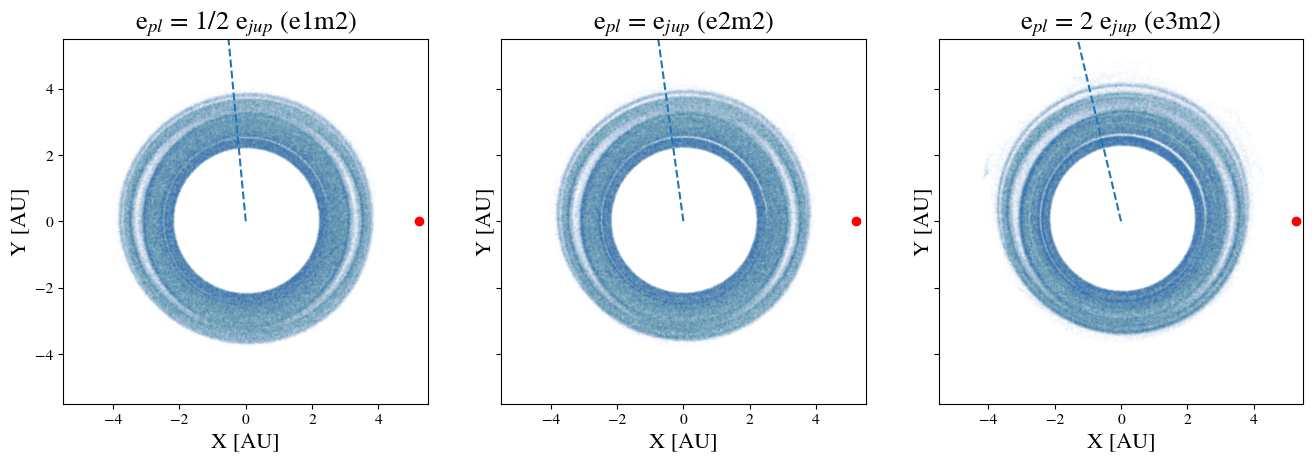
\includegraphics[width=\textwidth]{figures/xy.png}
    \caption{The positions of remaining planetesimals at the end of the CJ (left) and EJ (right) simulations. Jupiter's position is
    indicated by a red dot. Nonaxisymmetric features due to mean motion resonances are clearly visible in both cases. Higher
    order resonances are visible in the EJ case.\label{fig:xy}}
\end{figure*}

\section{Results} \label{sec:results}

We begin by examining the spatial distribution of planetesimals in the CJ and EJ simulations. The cylindrical position of the planetesimals 
in the the CJ and EJ simulations after 5000 years of integration are shown in the left and right hand panels of  figure \ref{fig:xy}, 
respectively. In the circular Jupiter case, a gap produced by the 2:1 MMR is visible, while the 3:1 and 5:3 MMR gaps are visible with an 
eccentric Jupiter. The non-axisymmetric nature of the gaps is due to the fact that planetesimals in the vicinity of the resonances have been 
excited onto non-circular orbits. Although the spatial distribution of planetesimals near MMR in debris disks may provide clues to detect 
unseen planets, we will not focus on this topic here, as it has already been covered in detail by other studies \citep{2016ApJ...818..159T, 
2018ApJ...857....3T}.

The MMRs are most clearly visible when viewing the semimajor axis and eccentricity distribution of the planetesimals. This is shown 
in figure \ref{fig:ae}. The top panel corresponds to the CJ simulation and the bottom panel corresponds to EJ. The solid vertical lines 
in this plot represent the nominal locations of the resonances. Near the nominal resonance locations, the a-e distribution of the 
planetesimals exhibits well-defined spikes which curve slightly inward due to conservation of the Jacobi energy. In the EJ simulation, 
the eccentricity distribution of bodies near resonance extends below the initial forced value. This is a reflection of the fact that the resonant 
angles of these bodies are undergoing libration, which drives periodic oscillations in both semimajor axis and eccentricity. The coupling 
between these two quantities is described by equation \ref{eq:tiss}. Because the strength of the resonances scales with the initial 
eccentricity of the planetesimals, the eccentricity spikes are larger in the EJ simulation. Additionally, the relative size of the 3:1 and 5:3 
MMR spikes also grows because the strength of a MMR scales as $e^{q}$, where $q$ is the order of the resonance 
\citep{1994PhyD...77..289M}.

\begin{figure}
    \begin{center}
    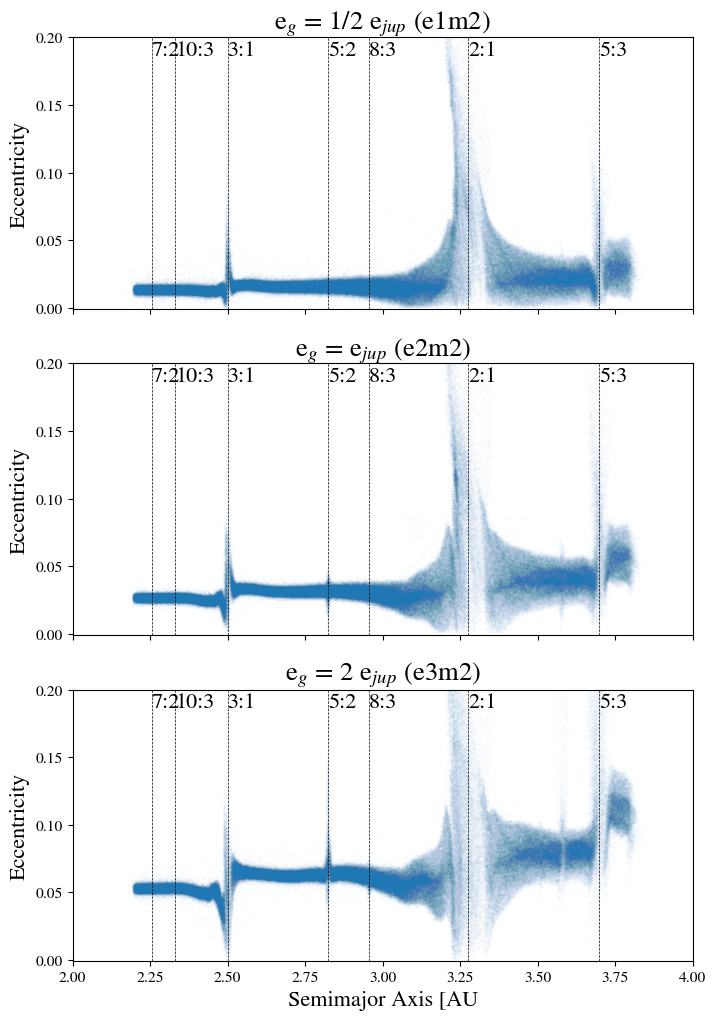
\includegraphics[width=0.4\columnwidth]{figures/ae.png}
    \caption{The semimajor axis - eccentricity state of the remaining planetesimals are shown at the end of the CJ (top) and EJ (bottom) 
    simulations. The vertical bars mark the nominal locations of prominent resonances. Planetesimals affected by resonance with Jupiter gain
     eccentricity, and due to conservation of the Jacobi energy, reduce their semimajor axes. This produces the curved fingerlike structure 
     extending off of the resonances. In the EJ case, some bodies in resonance take on eccentricities smaller than their initial forced values as 
     they undergo libration.\label{fig:ae}}
    \end{center}
\end{figure}

The MMRs have an additional important effect, which is to drive precession of the longitudes of perihelion of planetesimals. 
This effect becomes important in the EJ simulation because the orbits of bodies are initially aligned with that of Jupiter 
(see section \ref{sec:sec_force}). As is shown in figure \ref{fig:long_ph}, the strong precession induced by the MMRs overcomes the 
secular forcing and randomizes the orbital orientations of bodies near the resonances. The dashed horizontal lines in figure 
\ref{fig:long_ph} indicate the libration width (should probably show the equation I used to calculate this) of a planetesimal with an 
eccentricity of $e_{forced}$ at each resonance, which approximately shows the zone of influence of each MMR.

\begin{figure}
    \begin{center}
    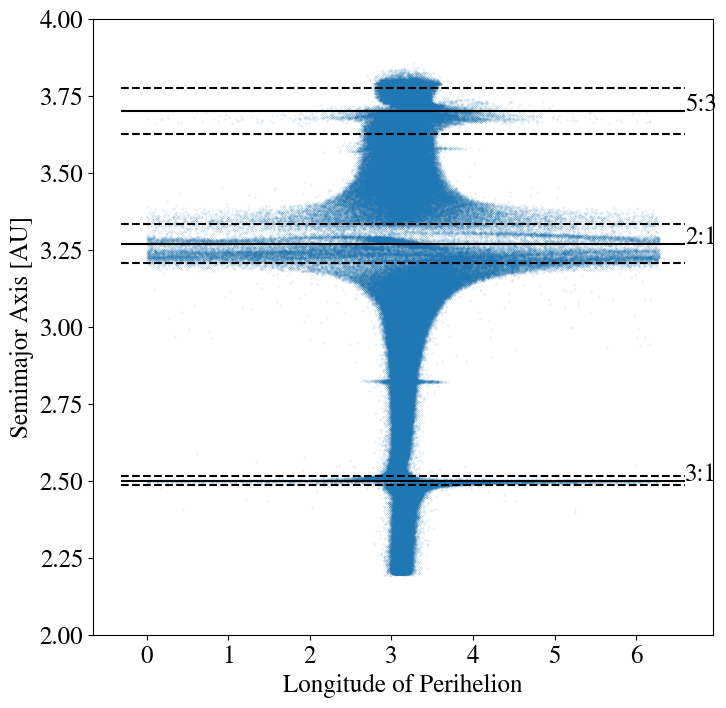
\includegraphics[width=0.4\columnwidth]{figures/long_ph.png}
    \caption{The semimajor axis and pericenter orientation of remaining planetesimals at the end of the EJ simulation. All bodies start with their 
    pericenters closely aligned with Jupiter's ($\varpi = \pi$). Near the resonances, bodies undergo strong precession which randomizes their 
    orbital orientations. Two-body interactions between the planetesimals in resonance and nearby non-resonant planetesimals drags their 
    longitude of perihelia along with.\label{fig:long_ph}}
    \end{center}
\end{figure}

\begin{figure}
    \begin{center}
    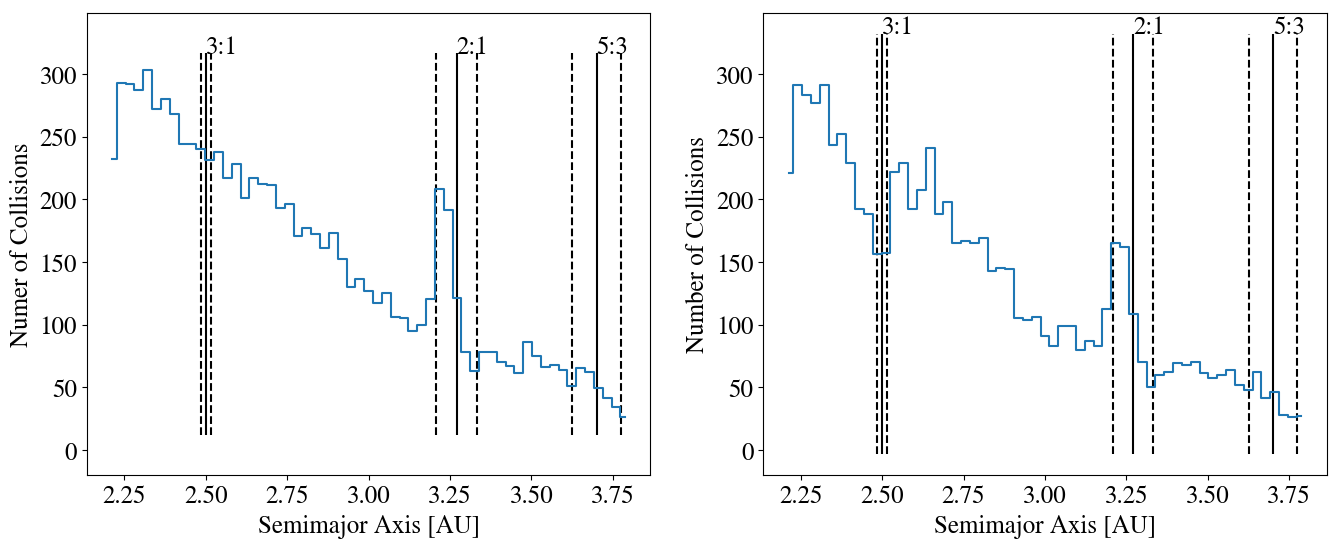
\includegraphics[width=0.4\columnwidth]{figures/coll_hist_a.png}
    \caption{A kernel density estimate (KDE) of the collision rate as a function of semimajor axis in the CJ (top) and EJ (bottom) simulations. 
    There are measureable changes in the collision rate near 2:1 and 3:1 MMRs, each of which produce qualitatively different changes in the 
    collision rate. The vertical bars mark the nominal locations of prominent resonances.\label{fig:coll_hist_a}}
    \end{center}
\end{figure}

\subsection{Collision Rates}\label{sec:coll_rates}

A prediction of the collision rate using the Safronov equation (eq \ref{eq:safronov}) and the positions and velocities of the planetesimals
suffers from an important limitation. As we will show below, the velocities of planetesimals near the MMRs does not follow a unimodal 
distribution. This makes it difficult to characterize the motion of the planetesimals with a single encounter velocity $v_{p}$ and so predicting 
the collision rate using a statistical approach is far from straightforward. This operation becomes even more complicated with a secularly 
perturbed disk where there is a transition between aligned and randomly oriented orbits near the interface of the resonances (see figure 
\ref{fig:long_ph}.

Figure \ref{fig:coll_hist_a} shows the semimajor axis of collisions resolved in the CJ (top) and EJ simulations (bottom). We define 
the semimajor axis of a collision as the semimajor axis of the first of the two planetesimals participating in a collision at the 
moment that it happens. To ensure that the definition of the first and second collider chosen by {\sc ChaNGa} does not influence 
these results, we also tried constructing figure \ref{fig:coll_hist_a} using the properties of the second collider and found no qualitative 
differences. Although both simulations were integrated and collisions were resolved for 5,000 years, we only show collisions that occurred 
during the last 3,000 years of the simulations. Before this time, the resonant features in the semimajor axis-eccentricity distribution (see 
figure \ref{fig:ae}) were still developing and had not yet reached a steady state (the libration timescale of the MMRs we are interested in 
turns out to be about 2,000 years). This results in transient features appearing in the collision profiles early on, which we exclude from 
figure \ref{fig:coll_hist_a} and all subsequent figures.

We find that the features present in figure \ref{fig:coll_hist_a} are highly sensitive to the choice of binning when constructing a standard 
histogram and instead model the occurrence of collisions as a function of semimajor axis using a kernel density estimate (KDE). We use 
the {\sc neighbors.KernelDensity} function from the {\sc sklearn} \citep{scikit-learn} package to construct our KDEs. For the kernel, we use 
a tophat function with a bandwidth of 0.01 AU.

Near some of the MMRs, there are noticeable suppressions or enhancements of the local collision rate. This contrasts with the findings of 
\citet{2000Icar..143...45R}, who simulated a similar setup and found no discernible features near the MMRs. We attribute the differences to 
a more careful treatment of timestepping in our simulations. Just interior to the 2:1 resonance, the collision rate is strongly enhanced. In the 
EJ simulation, there is a significant deficiency in the number of collisions near the 3:1 MMR. This feature, although still present, is much 
weaker in the CJ simulation. We attribute this to the fact that the strength of a second-order MMR scales as $e^{2}$, while a first order 
MMR scales with $e$ \citep{1994PhyD...77..289M}. One would therefore expect the 3:1 resonance to have more of an influence on the 
collision rate in a more eccentric disk. Although viewing the collision rate as a function of semimajor axis demonstrates a clear connection 
between the resonances and the collision rate, this does not immediately indicate where the dust generated by collisions will end up in the 
disk. (Why is the feature around the 3:1 MMR so different than the 2:1?)

\begin{figure*}
    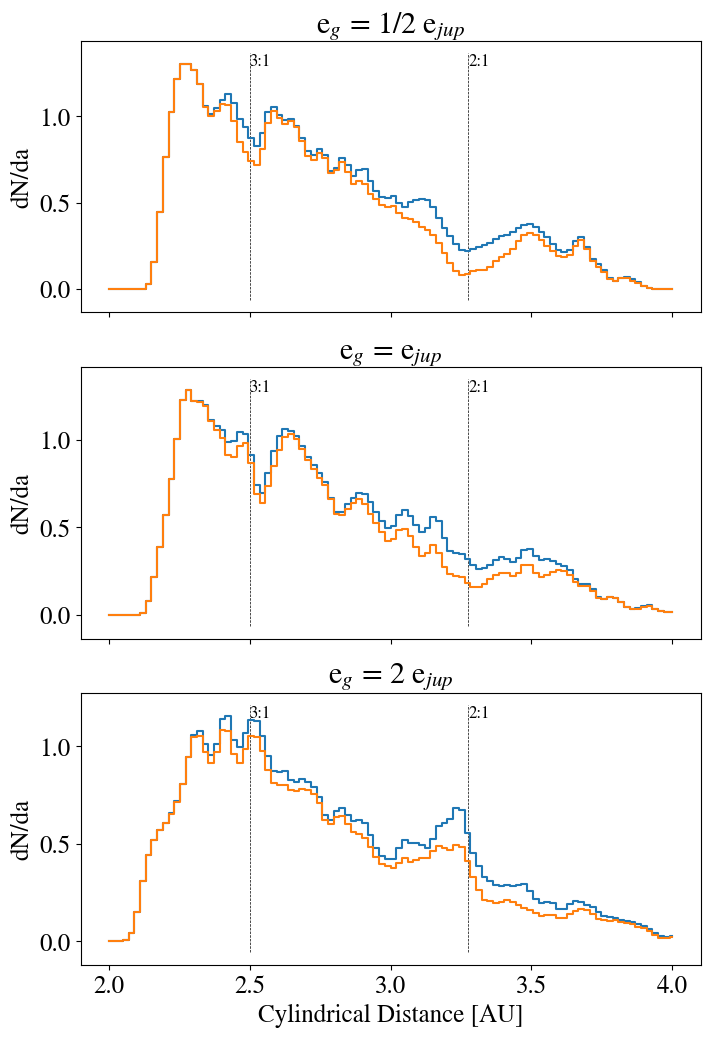
\includegraphics[width=\textwidth]{figures/coll_hist_r.png}
    \caption{\textit{Top:} A KDE of the collision rate in the CJ (left) and EJ (right) simulations as a function of cylindrical distance from the central 
    star. Vertical lines mark the nominal locations of the MMRs. Variations in the collision rate are visible near the MMRs, but are distinctly 
    different than the feature that appeared in figure \ref{fig:coll_hist_a}. \textit{Middle:} The azimuthally-averaged surface density of remaining 
    planetesimals. \textit{Bottom:} The cylindrical distance and eccentricities of remaining planetesimals. The cones extending upward from the 
    resonance locations are due to the fact that eccentric planetesimals explore a wide range of physical space over the course of an orbit.\label{fig:coll_hist_r}}
\end{figure*}

\subsection{Where Does the Dust End Up?}

To construct a radial dust profile, we begin by making the assumption that any dust generated by collisions is strongly coupled to the 
gas. For a dust grain larger than the mean free path of the gas particles, the timescale to damp its eccentricity is given by 
\citep{1976PThPh..56.1756A}

\begin{equation}\label{eq:t_edamp}
    t_{e, damp} = \frac{8 s \rho}{3 e C_{D} \rho_{g} v_{th}}.
\end{equation}

where $m$, $e$ and $s$ are the mass, eccentricity and radius of the dust grain. $C_{D}$ is a drag coefficient which is of order unity, $
\rho_{g}$ is the local density of the gas and $v_{th}$ is its thermal speed. At 3 AU, the gaseous component of the solar nebula has a 
density of $4 \times 10^{-10}$ g cm$^{-3}$ and a typical thermal speed of $10^{5}$ cm s$^{-1}$ \citep{1981PThPS..70...35H}. For a 1 
mm dust grain with a density of 1 g cm$^{-3}$ and an eccentricity of 0.05, the damping timescale is $4 \times 10^{-3}$ years. This is 
orders of magnitude smaller than the collision timescale, therefore we conclude that collisionally generated dust grains will immediately 
couple to the gas.

Operating under this assumption, a map of the relative concentration of second-generation dust can be constructed from the cylindrical 
distance at which the collisions occur. This is shown in the top panels of figure \ref{fig:coll_hist_r}, where the left side corresponds to the CJ 
simulation and the right side corresponds to EJ. As in figure \ref{fig:coll_hist_a}, a KDE of the collision rate is constructed using a tophat 
kernel with a bandwidth of 0.01 AU.

In contrast to what was seen in figure \ref{fig:coll_hist_a}, the radial collision rate is now suppressed near the 2:1 MMR. The spike in the 
collision rate at semimajor axes interior to this location becomes washed out when viewed instead by cylindrical distance because the 
spread in the eccentricities of the colliding planetesimals is so large. Although many of the collisions happen at the same semimajor axis, 
they occur at very different distances from the central star. The second row of figure \ref{fig:coll_hist_r} shows the azimuthally averaged 
surface density of the planetesimal disk at the end of the simulations. These profiles were calculated using the {\sc PYNBODY} analysis 
package \citep{2013ascl.soft05002P}.

In both the CJ and EJ simulations, the local minima in the surface density profiles match well with the minima in the collision rates. 
Additionally, the minima in the EJ simulation are offset from the centers of the resonances. This can be explained as follows: for 
planetesimals affected by the MMRs, the typical encounter velocity is large and gravitational focusing is suppressed. Here, the collision 
cross section is geometric. In this limit, the collision probability scales with the ratio between the geometric cross section of the 
planetesimals and the surface area of a sphere with radius $r$, where $r$ is the distance between the bodies and the central star. This 
ratio, and therefore the collision probability, is largest when $r$ is minimized (see \citet{2003AJ....125.2692L}). Therefore, the collision 
probability for planetesimals affected by resonance is smallest at aphelion. This is also consistent with the reduced surface density exterior 
to the resonances.

Finally, the bottom row of figure \ref{fig:coll_hist_r} demonstrates the difficulty with calculating the collision rate from the position and velocity 
distribution of particles. At a given distance from the central star, the distribution of velocities (using eccentricity as a proxy for encounter 
velocity), is not unimodal. In addition, the wings extending off of the resonances in these plots show that planetesimals can interact and collide 
with bodies far from the centers of the resonances. The bump seen in the collision rate in the EJ simulation around 2.7 AU is like a result of 
interaction between planetesimals in the 3:1, 5:2 and 2:1 resonances.

So far, we have shown that mean-motion resonances with a perturbing giant planet will produce measureable radial variations in the collision 
rates across a disk of planetesimals, which should give rise to variations in the dust profile. In addition, distinctly different features are 
produced if the giant planet is on an eccentric, rather than a circular orbit. In the next section, we would like to determine whether these 
features can be used to place any constraints on the mass and eccentricity of the planet.

\section{Influence of Jupiter's Mass and Eccentricity on the Radial Dust Profile}

\begin{figure*}
    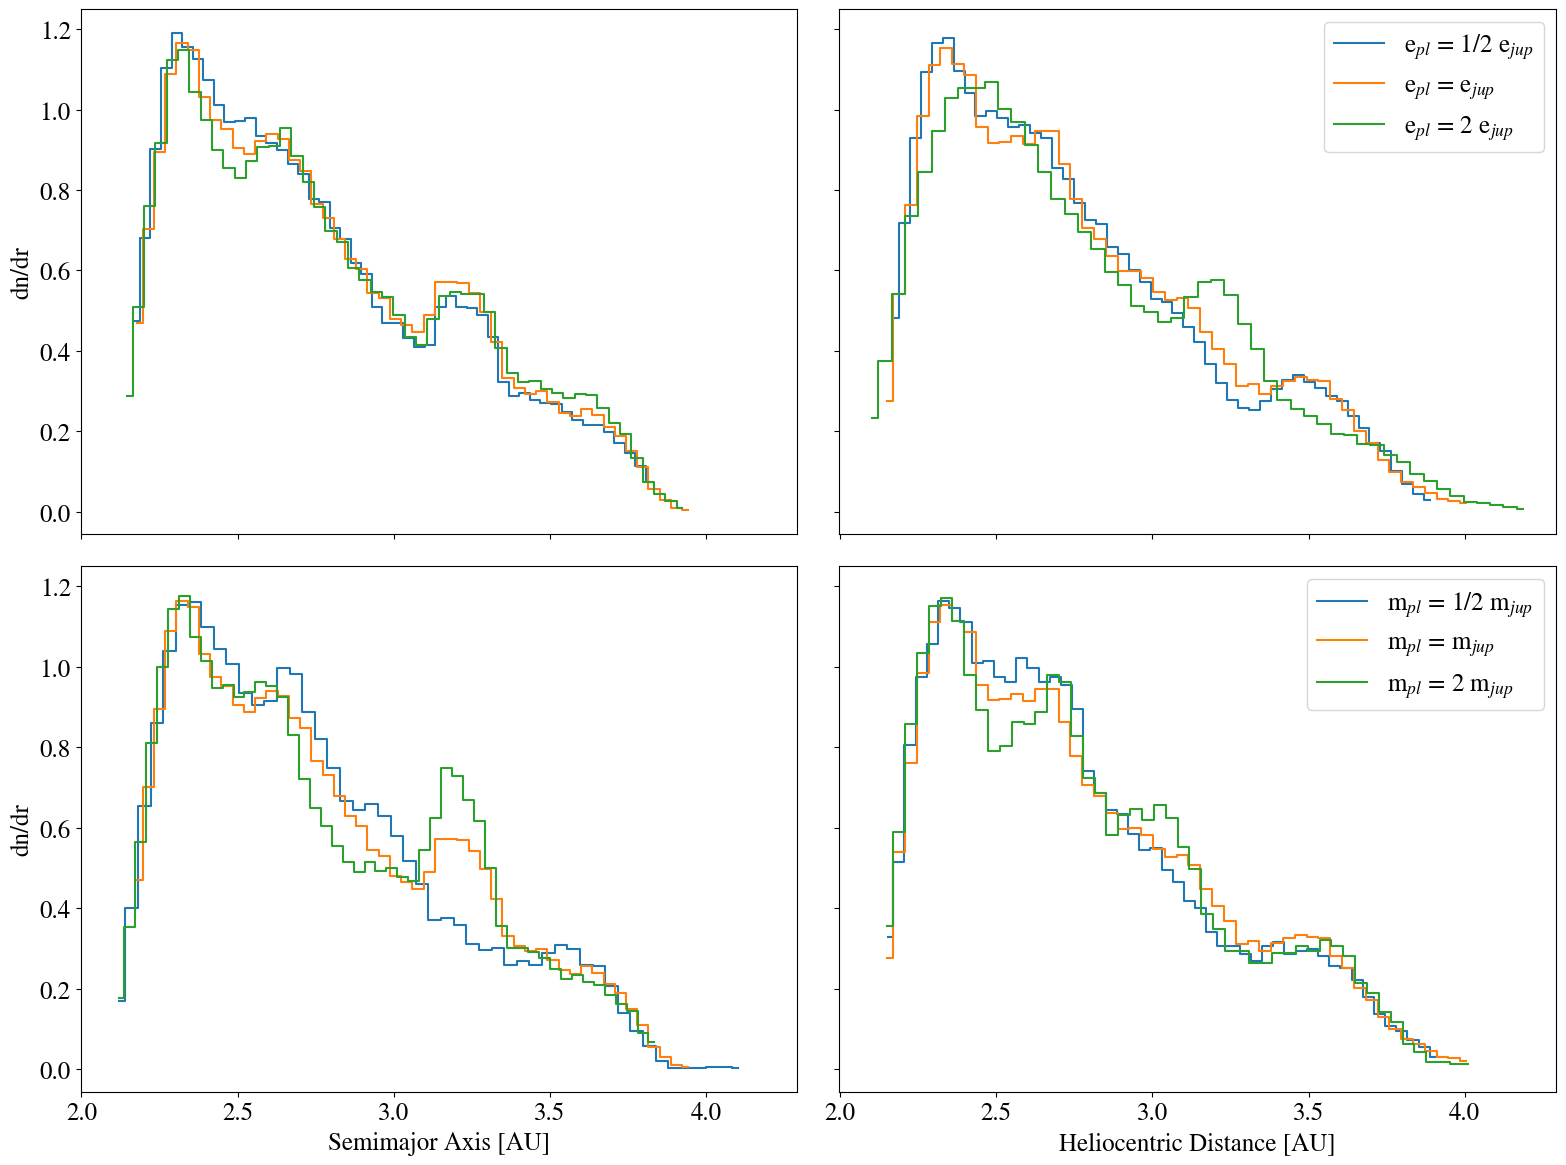
\includegraphics[width=\textwidth]{figures/coll_hist_e_and_m.png}
    \caption{\textit{Top}: KDE of the number of collisions at each semimajor axis (left) and heliocentric distance (right) as the eccentricity of of the perturbing planet is varied. \textit{Bottom}:  Same as top row, except the perturber's eccentricity is set to $e_{jup}$ and the mass is now varied. In all plots, the PDF is normalized to the ($e_{jup}, m_{jup}$) case. Characteristic bumps or dips appear near the 2:1 and 3:1 MMRs, the presence of which depends on the mass and eccentricity of the perturber. \label{fig:coll_hist_e_and_m}}
\end{figure*}

\begin{figure*}
    \begin{center}
    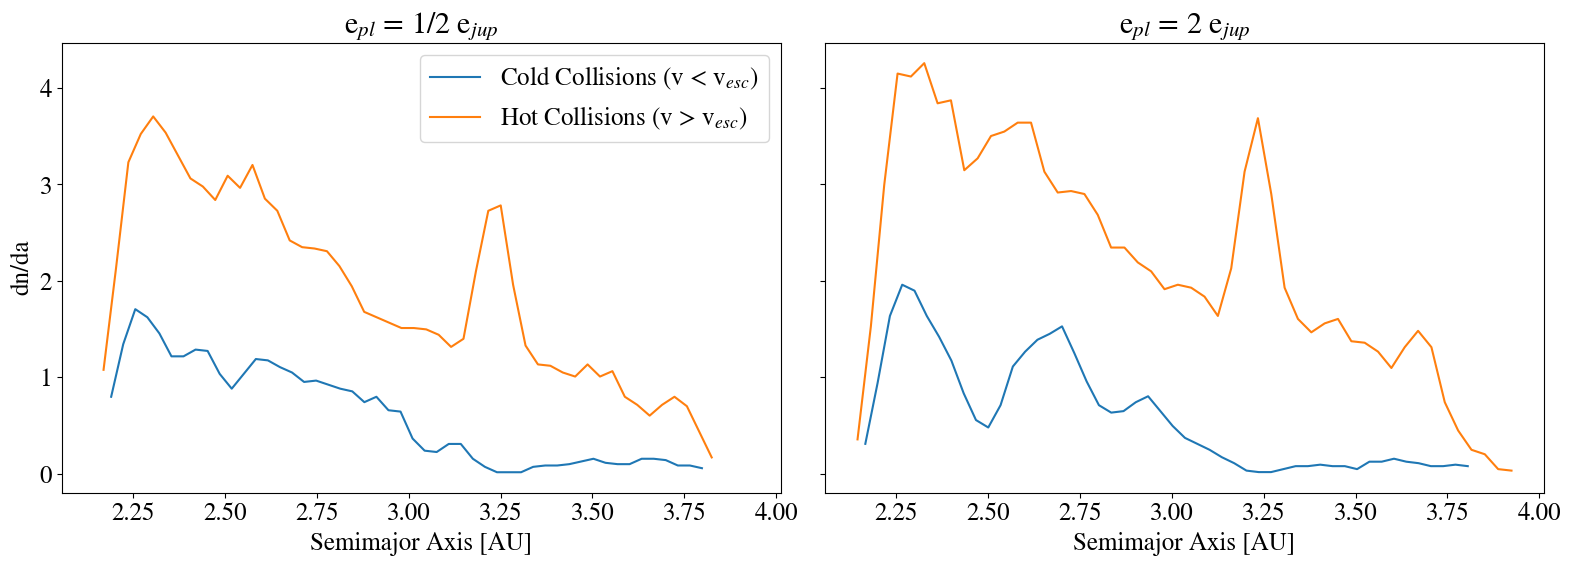
\includegraphics[width=\textwidth]{figures/coll_hist_hot_cold_a.png}
    \caption{KDE of the number of collisions at each semimajor axis for the lowest eccentricity case (left) and highest eccentricity case (right). To elucidate why a bump forms at the 2:1 while a dip forms at the 3:1 MMR, we split the resolved collisions into hot and cold categories. A bump is produced when the hot collision rate increases, while a dip is produced when the cold collision rate decreases.\label{fig:coll_hist_hot_cold_a}}
    \end{center}
\end{figure*}

\begin{figure*}
    \begin{center}
    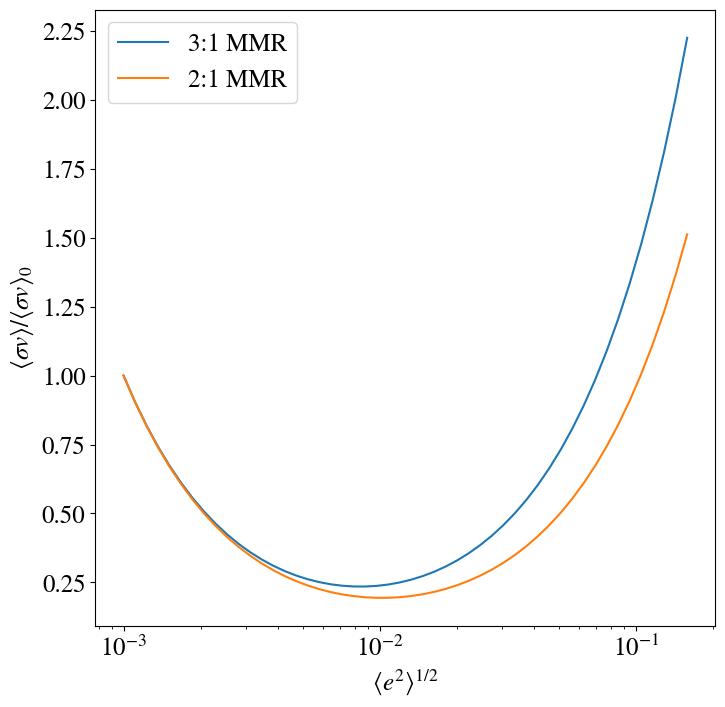
\includegraphics[width=0.4\textwidth]{figures/coll_gf_vary.png}
    \caption{The collision rate of a population of 300 km planetesimals as a function of the rms eccentricity in the vicinity of the 3:1 and 2:1 MMRs, relative to the value at $\left< e^{1/2} \right>^{2}$ = $10^{-3}$. The resonances will act to dynamically heat the local planetesimal population. The local minimum corresponds to the rms eccentricity at which the typical planetesimal encounter velocity is $v_{esc}$. If the planetesimals are heated by a small amount, gravitational focusing is suppressed and the collision rate decreases. Stronger dynamical heating will increase the encounter rate enough to overcome the lack of gravitational focusing.\label{fig:coll_gf_varg}}
    \end{center}
\end{figure*}

\begin{figure*}
    \begin{center}
    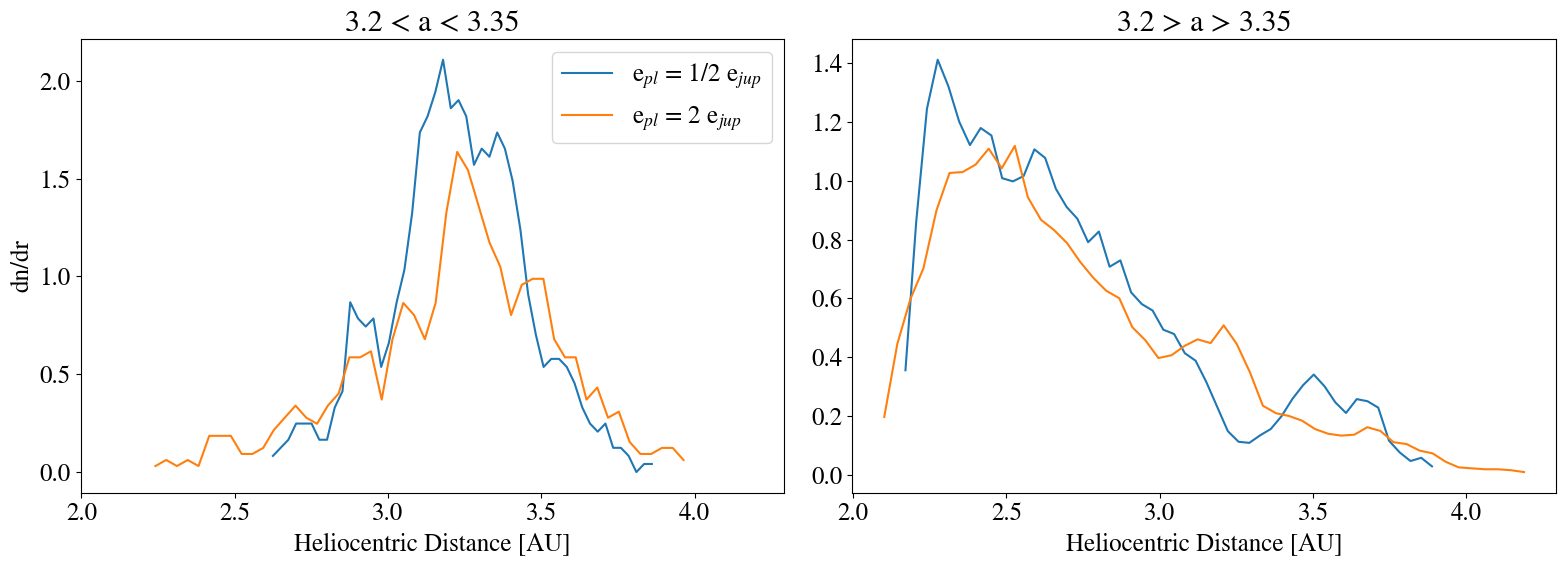
\includegraphics[width=\textwidth]{figures/coll_hist_r_inout_res.png}
    \caption{KDE of the number of collisions at a given heliocentric distance for planetesimals inside (left) and outside (right) of the 2:1 MMR. In the $e_{pl} = 2 e_{jup}$ case, a bump, rather than a dip appears near the 2:1 MMR (see figure \ref{fig:coll_hist_e_and_m}). This bump is produced by non-resonant planetesimals undergoing collisions near the center of the 2:1 MMR.\label{fig:coll_hist_r_inout_res}}
    \end{center}
\end{figure*}

\begin{figure*}
    \begin{center}
    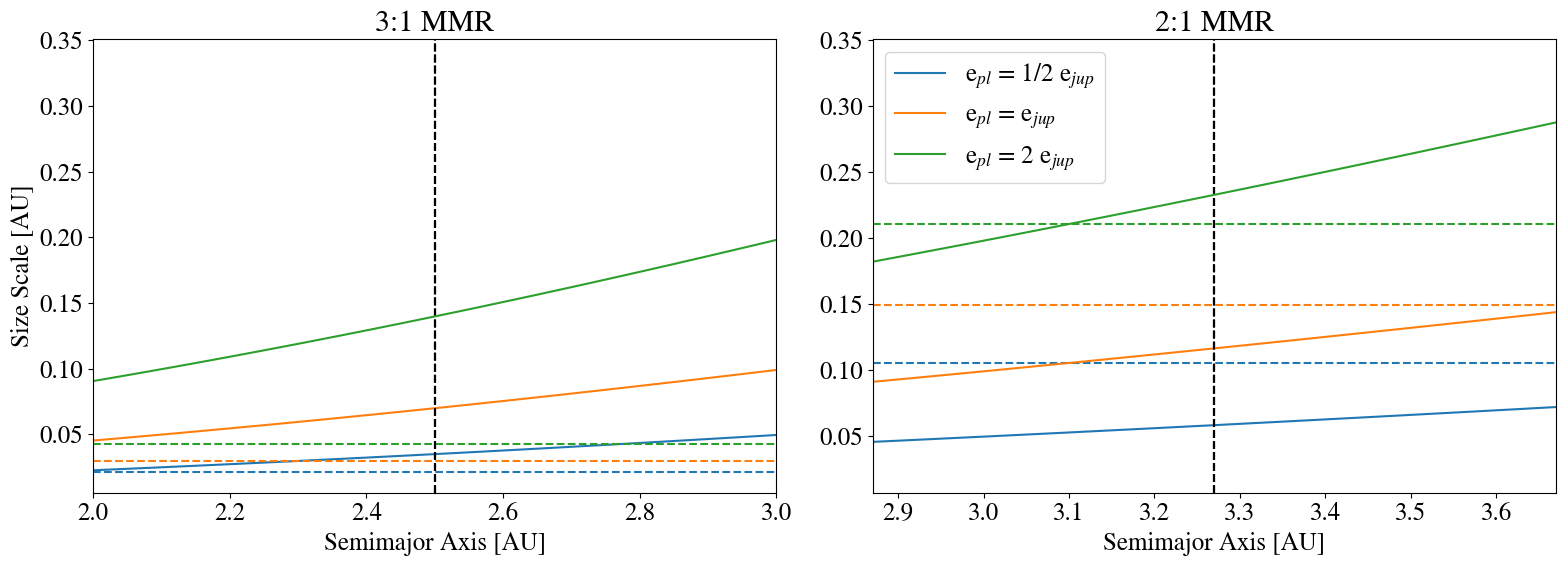
\includegraphics[width=\textwidth]{figures/wander_res_scale.png}
    \caption{The radial excursion distance of a planetesimal $\delta r_{ex}$ =  ($a_{pl} (1 + e_{f}$) (solid lines) near the resonance and full libration width $\delta r_{res}$ (dashed lines) of that resonance for the 3:1 (left) and 2:1 (right) MMR. For the 2:1 MMR, $\delta r_{ex} < \delta r _{res}$ near the resonance for $e_{pl} = 1/2 e_{jup}$ and $e_{pl} = e_{jup}$. In these case, a dip, rather than a bump appears near the resonance in the bottom right panel of figure \ref{fig:coll_hist_e_and_m}. \label{fig:wander_res_scale}}
    \end{center}
\end{figure*}

\section{Observability of Dust} \label{sec:dust}

Aaron's CASA images go here

\section{Summary and Discussion} \label{sec:discuss}

\bibliography{references}

\clearpage

\end{document}
